\documentclass[../main.tex]{subfiles}
\begin{document}

\section{Research Design}
This study adopts a mixed-method approach that integrates automated text analysis using a large language model (LLM) with traditional manual evaluation methods. The feasibility study is structured to assess the LLM's ability to evaluate administrative acts by comparing its outputs against those generated by human experts. The overall framework comprises data collection, checklist integration, automated querying, and performance benchmarking. 

To structure the automation process and facilitate independent testing, we conceptualized the core LLM-driven tasks as two distinct functional components, referred to here in a simplified sense as "agents". Each agent is designed to perform a single, specific action within the overall administrative control workflow. This separation allowed for a focused evaluation of the LLM's effectiveness in executing each sub-task individually.

The first agent is responsible for checklist selection. Its function is to analyze the content of an administrative act ("determina") and identify the most appropriate checklist from the predefined set, based on the descriptions and criteria embedded within each checklist's JSON definition. The second agent handles the checklist completion task. Once a checklist is selected (either manually for testing or by the first agent), this second agent systematically processes each point, querying the LLM to evaluate the determination against the specific instruction and criterion of that point, ultimately providing a compliance assessment (e.g., "SI", "NO", "NON PERTINENTE").

This modular design, while simplifying the initial feasibility study and enabling targeted performance analysis, represents an intermediate step. The intention for a future, fully integrated system is to combine these functionalities into a single, more sophisticated agent. This unified agent would autonomously perform the entire sequence: reading and understanding the administrative act, selecting the correct checklist, and then proceeding to complete the evaluation point by point, thereby fully automating the core assessment process.

\section{Workflow Diagram}
A workflow diagram (Figure \ref{fig:workflow}) summarizes the entire process that has been done. 

\begin{enumerate}
    \item \textbf{Data Collection:} Download PDFs and extract text.
    \begin{enumerate}
        \item Download the "Determine" (i.e. the acts the we want to analyze) 
        \item Preprocess the PDF files
        \item Gather the Municipality Checklists: Gather all the necessary checklists from the municipalities
    \end{enumerate}
    \item \textbf{LLMs agents:} This was the main focus of the study
    \begin{enumerate}
        \item \textbf{Choose the right checklist for the act} : The llm agent chooses the right checklist needed for the act based on the content of the act and the description of the checklist
        \item \textbf{Evaluate Checklist Points} : the agent answer every point of the checklist
    \end{enumerate}
    \item \textbf{Analysis of the result}: Main block that will be discussed in the next Chapter (Ch \ref{ch:Results})
    \begin{enumerate}
        \item Gather all the response from all the LLMs agents
        \item Process the results from the LLMs
        \item Compare LLMs responses to Human Evaluation
    \end{enumerate}

\end{enumerate}

\begin{figure}[H]
    \caption{The architecture and workflow followed}
    \label{fig:workflow}
    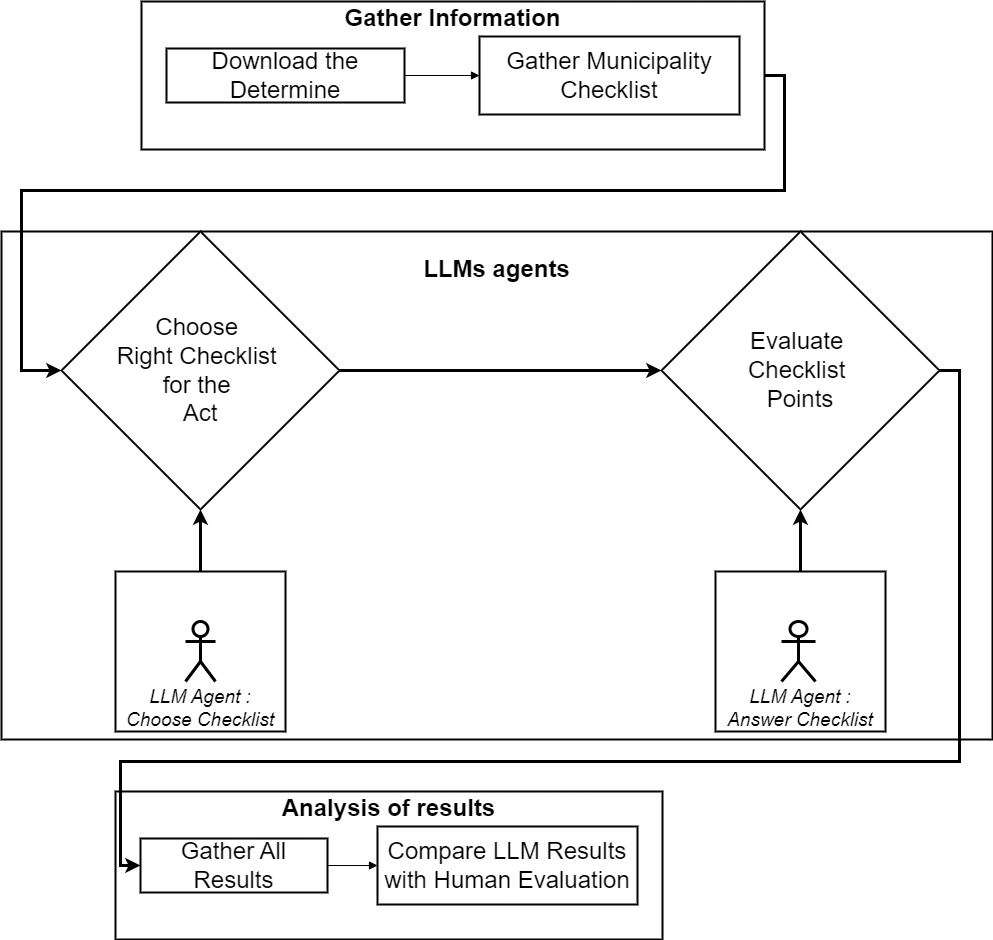
\includegraphics[width=10cm]{Graphs/0.Workflow.png}
\end{figure}

\section{Data Collection Process}
Municipal documents, specifically determinations (or “determina”) available on the public bulletin (or "albo pretorio"), form the primary data source. For each document, the following steps are undertaken:

\begin{itemize}
    \item \textbf{Document Acquisition}: Download PDF files of relevant determinations.
    \item \textbf{Text Extraction}: Convert each PDF into plain text using Python-based tools, ensuring the content is accessible for further processing.
    \item \textbf{Checklist Selection}: Use a CSV file that maps the document names to their associated checklists.
\end{itemize}

\subsection{Checklists Integration}
To standardize the evaluation process, a series of checklists was compiled based on the administrative control requirements used by public administration entities. These checklists were transformed into a JSON format, allowing the division of each checklist into individual questions. Each checklist point includes specific instructions that guide the evaluation of the act in question. In the \hyperref[appendix:json_template]{Appendix} there is the template for the JSON that is used in this study (see Appendix \ref{appendix:json_template}).

\section{LLMs agents}
\subsection{LLMs Usage}
The LLMs are central to this study. Its role is to analyze the text extracted from municipal determinations and respond to each point of the checklist. The process involves:

\begin{itemize}
    \item \textbf{Prompt Design and Configuration:}
    
 A structured prompt template was created to guide the LLM. The template includes:
    \begin{itemize}
        \item Instructions to the model as an expert in administrative law.
        \item A clear layout where each checklist point is presented as a question.
        \item A predefined answer format (e.g., SI/NO/NON PERTINENTE with a brief explanation if needed).
    \end{itemize}
    \item \textbf{Extraction and Analysis Process:}
    
 The LLM is queried for each checklist point using the custom prompt. The responses, initially in long text form, are processed using regular expressions to extract the essential output: namely, a categorical answer (SI, NO, NON PERTINENTE) and a concise explanation when necessary. A Python script orchestrates this process and aggregates the results into a CSV file.
    \item \textbf{Human Evaluation Procedure for Benchmarking:}
    
 To benchmark the LLM's performance, a parallel manual evaluation was conducted. A human expert compiled a checklist-based assessment for each determination. The automated results were then compared against these manually obtained values to assess accuracy and reliability.
\end{itemize}

\subsection{LLM Agent : Choose Checklist}

\subsubsection{Design Choices}
\label{subsubsec:choose_designchoices}

Developing the agent responsible for selecting the appropriate checklist for a given administrative act involved several key considerations, particularly regarding prompt structure and model configuration.

One primary investigation focused on the optimal placement of the administrative act's text ("determine") within the prompt structure provided to the LLM. Two main approaches were considered: placing the "determina" text within the initial system/developer prompt alongside the core instructions, or including it within the user prompt immediately preceding the specific question about checklist selection. Preliminary experiments indicated that placing the "determina" text directly within the user prompt yielded more accurate checklist selection results for the models tested in this specific task context. Consequently, this structure was adopted for the main experiments involving checklist selection.

Furthermore, to assess the robustness and generalizability of the selection capability, different Large Language Models were employed (e.g., comparing models like "gpt-4o-mini", "gpt-4o"...). Performance variations across models were analyzed to understand the impact of model size and architecture on this specific administrative task.

The influence of the "temperature" parameter was also explored systematically. Recognizing that the review of administrative checklists can sometimes involve a degree of interpretation or discretion by the human operator, different temperature settings (e.g., ranging from 0.0 for maximum determinism to 1.0 for increased variability/creativity) were tested. The aim was to investigate whether higher temperatures might allow the LLM to better handle nuances or borderline cases in act classification, while lower temperatures were expected to yield more consistent and predictable selections. This exploration helped in identifying the optimal balance between reliability and flexibility for the checklist selection agent.


\subsubsection{Prompt}
The prompt designed for the checklist selection agent also employed a two-part structure, assigning specific instructions to the system/developer role and the core query to the user role. 

The system prompt established the LLM's persona as an expert in administrative law, tasked with supporting a municipal employee by identifying the correct checklist to apply to a given administrative determination (determina). Crucially, the system prompt contained a detailed, multi-step procedure for the LLM: first, to read the different checklists provided (specifically, their names and detailed descriptions, which were dynamically inserted into the prompt); second, to read the full text of the determina; third, to carefully consider which checklist description best matched the content and purpose of the act; and finally, to respond only with the name of the selected checklist, potentially followed by brief explanatory notes. The list of available checklists, along with their NomeChecklist and detailed Descrizione (purpose, context, application criteria) fields from the structured JSON checklist file (e.g., checklists\_Lucca.json, checklists\_Olbia.json), was explicitly provided within this system prompt to serve as the basis for the selection. 

The user prompt then presented the actual task: it asked "A QUALE CHECKLIST APPARTIENE LA SEGUENTE DETERMINA?" (Which checklist does the following determination belong to?), reiterated the strict output format (only the name of one of the provided checklists, plus optional notes), and then presented the full text of the determina itself. This design aimed to leverage the LLM's text comprehension abilities to match the administrative act's content against the functional descriptions of the checklists provided in the system prompt, thereby automating the selection process based on predefined criteria.



\subsection{LLM Agent : Answer Checklist}

\subsubsection{Design Choices}

The second agent developed in this study is responsible for the core task of evaluating an administrative act against the points of a selected checklist. This involved designing an automated workflow to interact with the LLM for each checklist item and systematically testing different configurations.

From an implementation perspective, this agent iterates through each point defined in the selected checklist's JSON structure. For every point, a specific prompt is generated using the structure detailed previously (Section \ref{subsubsec:choose_designchoices}). This prompt incorporates the system instructions defining the LLM's role, the text of the administrative act ("determina"), and, crucially, the specific text ("Punto") and accompanying interpretation guidelines ("Istruzioni") for the checklist item currently under evaluation. The "ChecklistCompiler.py" script orchestrates this process.

Similar to the checklist selection agent, the checklist completion agent was tested using various LLMs of different sizes and capabilities (e.g., "gpt-4o-mini" vs. "gpt-4o") to assess the impact of model scale on this more granular question-answering task. A range of temperature settings (e.g., 0.0, 0.01, 0.2, 0.5, 1.0) was also systematically evaluated. Lower temperatures were hypothesized to promote consistency and adherence to the checklist instructions, while higher temperatures were explored to see if they could better handle potential ambiguities or nuances in the administrative text requiring more flexible interpretation, mirroring the discretion a human evaluator might apply.

A critical step in the implementation involved processing the LLM's responses. Since the models often generate verbose explanations alongside their core answer, a response parsing mechanism using regular expressions was implemented (ref. "analize\_response" method in "ChecklistCompiler.py" ). This function extracts the essential categorical evaluation (SI, NO, or NON PERTINENTE) from the model's output text. Standardizing the output in this manner was necessary to enable quantitative comparison against the ground truth evaluations provided by human experts, as detailed in the Results chapter (Chapter~\ref{ch:Results}). The effectiveness of this agent across the different configurations was then rigorously benchmarked using metrics such as accuracy and balanced accuracy (Section ~\ref{sec:performance_metrics}).


\subsubsection{Prompt}
The prompt engineering for the checklist completion agent utilized a structured two-part format, defining distinct roles for the system (developer) and the user, as specified in the prompt template file. 

The system prompt was designed to establish the LLM's persona as an expert assistant in Italian administrative law, tasked specifically with verifying the administrative regularity of a director's determination (determina) against provided checklist points. This system prompt included detailed, step-by-step instructions for the LLM: read the checklist point and its instructions, read the full determination text (which was embedded within this system prompt), verify compliance, and respond using one of the predefined categories: "SI" (compliant), "NO" (non-compliant, potentially indicating severity), or "NON PERTINENTE" (not relevant, with a brief explanation). It explicitly requested simple, clear language and an ordered response format. 

The user prompt, conversely, was dynamic for each checklist item. It provided the specific context for the query by injecting the checklist point's text (Punto), its detailed interpretation instructions (Istruzioni), and its unique identifiers (num, Sezione if applicable). Crucially, the user prompt also reinforced the desired output structure by explicitly requesting the answer in the format "RISPOSTA GENERALE : [SI, NO, NON PERTINENTE], [spiegazione sintetica se necessaria]". This dual-prompt structure aimed to clearly define the agent's role, task, and constraints while providing the specific details needed for evaluating each individual checklist requirement against the administrative act.   


\section{Models Used}
\label{subsec:models}
This study employed a range of Large Language Models (LLMs) and software libraries to implement and evaluate the automated administrative checklist verification system.

To assess the feasibility and performance variations, several state-of-the-art LLMs from different families and sizes were investigated. The selection included models from OpenAI, Meta, and Mistral AI. Specifically, the following models were evaluated:

\begin{itemize}
    \item \textbf{OpenAI GPT Series}: 
        \begin{itemize}
            \item "gpt-4o"
            \item "gpt-4o-mini" 
        \end{itemize}
        These proprietary models were accessed via the official OpenAI API.
        
    \item \textbf{Meta Llama Series} :
        \begin{itemize}
            \item "llama 3.1 8B Instruct"
            \item "llama 3.1 70B Instruct"
            \item "llama 3.2 3B Instruct"
            \item "llama 3.3 70B Instruct"
        \end{itemize}
        These open source models represent different sizes and versions within the Llama family.
        
    \item \textbf{Mistral AI Series}:
        \begin{itemize}
            \item "Mistral v0.3 7B Instruct"
        \end{itemize}
        This open source model was the only one in the family that was tested.
\end{itemize}

A key practical consideration involved running the open source models locally. The 70-billion parameter Llama models ("llama-3.1-70B" and "llama-3.3-70B") exceed the memory capacity of typical research GPUs in their standard precision formats (FP16). To address this, these larger models were loaded using \textbf{4-bit quantization}. Quantization reduces the memory footprint and computational requirements by representing the model's weights with lower precision (4 bits per parameter instead of 16 or 32), enabling them to fit within the available GPU memory resources, albeit with a potential trade-off in prediction accuracy that this study implicitly evaluates through its comparative results\cite{gholami2021surveyquantizationmethodsefficient,li2024evaluating}.

\section{Libraries Used}
\label{subsec:libraries}
The implementation of the experimental workflow, including data processing, prompt generation, model interaction, and evaluation, relied primarily on Python and its ecosystem of libraries. The key libraries used for interacting with the LLMs were:

\begin{itemize}
    \item \textbf{Hugging Face "transformers"} Library: This library was essential for loading, configuring, and running the open-weight models (Llama and Mistral series) locally on the available hardware. It provides a standardized interface for accessing pre-trained models and managing tasks like text generation and quantization.
    \item \textbf{OpenAI Python Client Library}: Interaction with the proprietary GPT models ("gpt-4o" and "gpt-4o-mini") was managed using the official OpenAI API and its corresponding Python client library. This allowed for sending prompts and receiving generated checklist evaluations from OpenAI's servers.
\end{itemize}

Other Python libraries were used for auxiliary tasks such as text extraction from PDFs, data manipulation (e.g., "pandas"), regular expression processing for response parsing ("re"), and file handling. The evaluation metrics were computed using the "scikit-learn" library.


\section{Implementation Challenges}
During implementation, several challenges were encountered:

\begin{itemize}
    \item \textbf{Text Extraction Issues:}
 Converting PDFs to clean text sometimes resulted in formatting problems or loss of information.
    \item \textbf{Prompt Engineering:}
 Designing prompts that reliably guided the LLM was iterative; adjustments were made to ensure clarity and precision in the responses.\cite{vatsalSurveyPromptEngineering2024}
    \item \textbf{Regex Limitations:}
 Extracting the standardized SI/NO/NON PERTINENTE responses from long texts required robust regular expressions, which sometimes needed fine-tuning to accommodate unexpected output variations.
    \item \textbf{Model Variability:}
 Different temperature settings and model sizes influenced the consistency of outputs, necessitating multiple pilot tests.
\end{itemize}
 


\section{Pilot Tests}
Before finalizing the experimental setup, several pilot tests were conducted:

\begin{itemize}
    \item \textbf{Hyper-Parameter Tuning:}
 Experiments with various temperature settings helped determine the optimal balance between creativity and consistency in responses.
    \item \textbf{Validation:}
 Initial tests compared the LLM’s responses with a small set of manually evaluated documents to fine-tune the prompt design and extraction process.
    \item \textbf{Iterative Refinement:}
 Feedback from pilot tests led to improvements in the prompt template, regex patterns, and overall processing pipeline, ensuring that the final system was robust and reliable.
\end{itemize}


% Include bibliography only when compiling this subfile independently
\ifSubfilesClassLoaded{
    \bibliographystyle{sapthesis}
    \bibliography{Tesi}
}{}

\end{document}